\documentclass[paper=letter, fontsize=12pt]{article}

\usepackage{amsmath,amsfonts,amsthm, amssymb} % Math packages
\usepackage{stmaryrd}
\usepackage[shortlabels]{enumitem}
\usepackage[pdftex]{graphicx}
\usepackage{booktabs}
\usepackage{placeins}
\usepackage{algpseudocode}
\usepackage[margin=1in]{geometry}
\usepackage{listings}
\usepackage{mdframed}
\usepackage{tcolorbox}
\usepackage{float}
\usepackage{subcaption}
\usepackage{url}
\usepackage{hyperref}

\usepackage{mathtools}
\DeclarePairedDelimiterX{\norm}[1]{\lVert}{\rVert}{#1}
\DeclarePairedDelimiterX{\abs}[1]{\lvert}{\rvert}{#1}
\DeclareMathOperator*{\argmin}{arg\,min}
\DeclareMathOperator{\spn}{span}
\DeclareMathOperator{\rct}{rect}
\DeclareMathOperator{\support}{support}
\DeclareSymbolFont{matha}{OML}{txmi}{m}{it}% txfonts
\DeclareMathSymbol{\varv}{\mathord}{matha}{118}
\DeclareMathOperator{\E}{\mathbb{E}}
\DeclareMathOperator{\Tr}{Tr}

\newcommand{\ceil}[1]{\lceil #1 \rceil}
\newcommand{\floor}[1]{\lfloor #1 \rfloor}
\newcommand{\Lapl}{\mathcal{L}}
\newcommand{\reals}{\mathbb{R}}
\newcommand{\complexes}{\mathbb{C}}
\newcommand{\ints}{\mathbb{Z}}
\newcommand{\innerp}[2]{\langle #1, #2 \rangle}
\newcommand{\vecii}[2]{\begin{bmatrix} #1 \\ #2 \end{bmatrix}}
\newcommand{\veciii}[3]{\begin{bmatrix} #1 \\ #2 \\ #3 \end{bmatrix}}
\newcommand{\rect}[1]{\rct \left( #1 \right)}
\newcommand{\pw}[1]{\begin{cases} #1 \end{cases}}
\newcommand{\Mod}[1]{\ \text{mod}\ #1}
\newcommand{\sumN}{\sum\limits_{n=0}^{N-1}}
\newcommand{\sumK}{\sum\limits_{k=0}^{N-1}}
\newcommand\given[1][]{\:#1\vert\:}

\graphicspath{{img/}}

\title{CS 543 - Final Project Proposal}
\author{
        Dario Aranguiz \\
        Cu-Khoi-Nguyen Mac
        }
\date{\today}


%%% Begin document
\begin{document}
\maketitle
% \pagebreak

\section{List of Group Members}

Our group consists of two members: Dario Aranguiz, a first year Master's
student working under Minh Do, and Khoi-Nguyen Mac, a first year Ph.D. student
also working under Minh Do.


\section{Project Description and Goals}

For our final project, we plan on implementing and exploring extensions of the
2015 paper \textit{Multimodal Deep Learning for Robust RGB-D Object
Recognition} \cite{Eitel2015} by Eitel et al. Our research group has recently
taken interest in the capabilities of depth cameras, and as such we have
various time of flight and structured-light depth sensors. Our group members
have done quite a bit of work in facial recognition and related areas using
depth, but an area we have yet to explore is augmenting traditional RGB-based
object recognition approaches with depth information. To this end, we have
chosen a recent paper from IROS 2015 that approaches the age-old problem of
object recognition with two new modalities, depth and deep learning.

The motivation for this technique is as follows. Convolutional Neural Networks
(CNNs) have proven remarkably useful for object recognition in the last few
years, with large companies such as Microsoft and Google pouring resources
into training more efficient networks. We are also interested in this problem,
but unlike Microsoft and Google, we do not have a GPU farm at our disposal to
train networks ad-infinitum. This prompts an interesting question; how can we
utilize pre-trained ImageNet networks while incorporating depth information?
CNNs require a fixed-size input, and most pre-trained networks have only been
trained on three-channel information. That constraint is the primary
motivation behind Eitel et al's technique.

To get around this problem, two separate three-channel networks are used: one
to process the incoming RGB images, and another to process the incoming depth
information. This depth information is transformed from single-channel
distance information to a three-channel RGB image using a depth-to-color
heatmap, the intuition being that useful features such as edges and corners
are preserved in this transformation. The final fully-connected layers of each
of these networks are then removed, and the second-to-last activation layers
are fed into a single large classification layer, merging the two networks.
Additional preprocessing is also done, but the system functions loosely as
described.

Our expected final outcome is to have a fully-functioning system that can
distinguish between objects from the Washington RGB-D Object Dataset. At
minimum, we aim to replicate the paper and get a recognition system of our own
running locally. We have a few stretch goals, listed in order of expected
difficulty:

\begin{enumerate}

    \item \textbf{Different Backends} - The current most-frequently used
    network backend is a package called Theano. However, Google recently
    released their own open-source Machine Learning backend called
    TensorFlow. It would be interesting to compare the efficacy of these two
    systems with our project.

    \item \textbf{Different Classification Layers} - In the paper, the authors
    recommend using a single fully-connected layer at the end of the pipeline
    for classification. It would be interesting to see how this scheme
    compares with other classification methods such as logistic regression,
    SVM, Random Forests, and others.

    \item \textbf{Different Preprocessing Schemes} - The authors prescribe a
    number of preprocessing techniques to convert depth images from one-channel
    data to three-channel data, but other preprocessing techniques have been 
    used in the past to do this as well. 

    \item \textbf{Network Modifications} - This is by and large our most
    ambitious stretch goal. The two-network system is core to the authors' 
    architecture, but we would be interesting in exploring different ways of 
    fusing depth data with traditional RGB data. This comes with a number of
    challenges, the least being that any modification to a pretrained ImageNet
    network would eliminate the benefit of using a pretrained network at all.

\end{enumerate}


\section{Member Roles}

While not exactly amenable to modularization, this project can be loosely split
into three different sections: preprocessing, classification layer, and network
setup. Dario will own the preprocessing stage, and Mac will own the
classification layer, while we will equally share the load for programming the
network and training.


\section{Resources}

For our data, we will be utilizing the Washington RGB-D
Object Dataset. Researchers at the University of Washington have compiled a
dataset of 300 common household objects, scanned on a turntable at 640x480
resolution. These images are all segmented, although the image sizes have yet to
be normalized. Figure \ref{fig:washington_samples} illustrates two samples of the dataset, being an apple and a banana. Each sample comes with an RGB image, a depth map, and a mask to segment the object.

\begin{figure}[htbp]
	\centering
	\begin{subfigure}[b]{0.32\linewidth}
		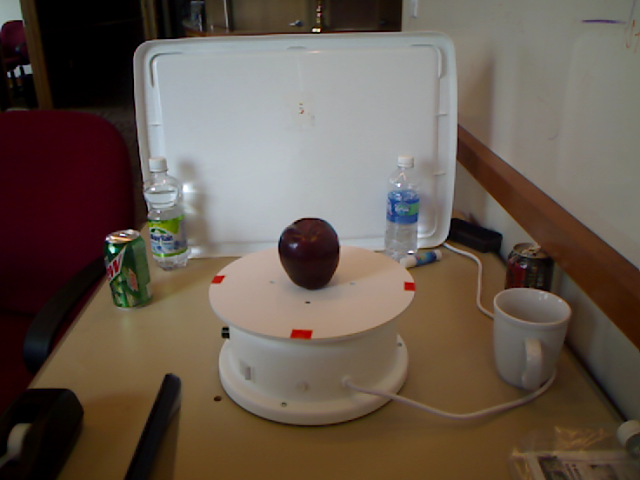
\includegraphics[width=\textwidth]{apple_1_1_100}
		\caption{Apple - color}
	\end{subfigure}
	\begin{subfigure}[b]{0.32\linewidth}
		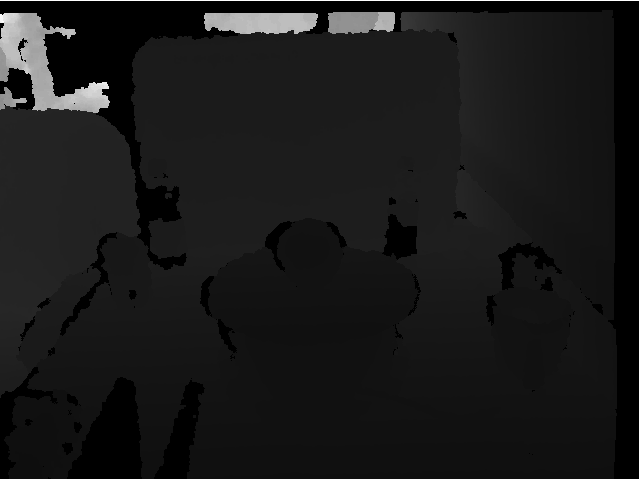
\includegraphics[width=\textwidth]{apple_1_1_100_depth_n}
		\caption{Apple - depth}
	\end{subfigure}
	\begin{subfigure}[b]{0.32\linewidth}
		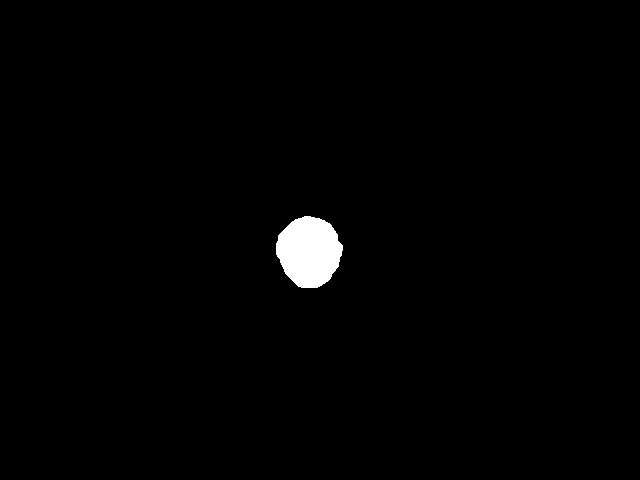
\includegraphics[width=\textwidth]{apple_1_1_100_mask}
		\caption{Apple - mask}
	\end{subfigure}
	\\
	\begin{subfigure}[b]{0.32\linewidth}
		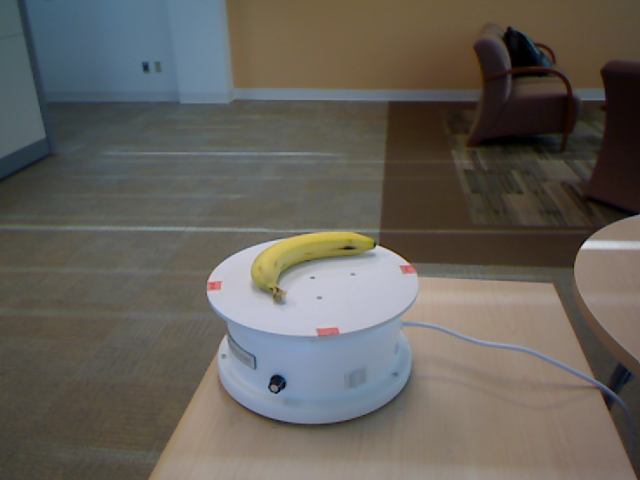
\includegraphics[width=\textwidth]{banana_1_1_100}
		\caption{Banana - color}
	\end{subfigure}
	\begin{subfigure}[b]{0.32\linewidth}
		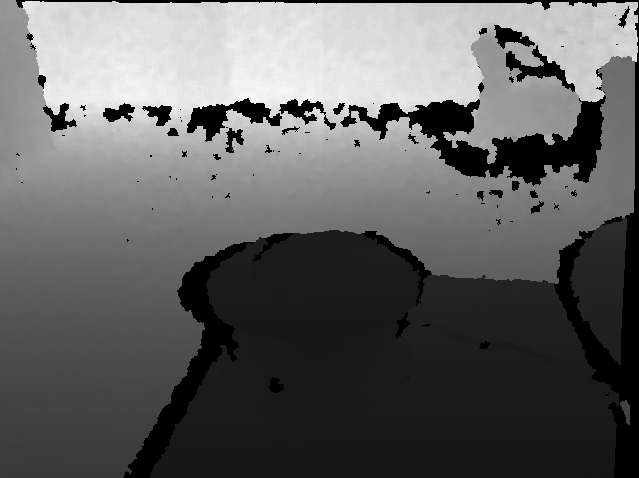
\includegraphics[width=\textwidth]{banana_1_1_100_depth_n}
		\caption{Banana - depth}
	\end{subfigure}
	\begin{subfigure}[b]{0.32\linewidth}
		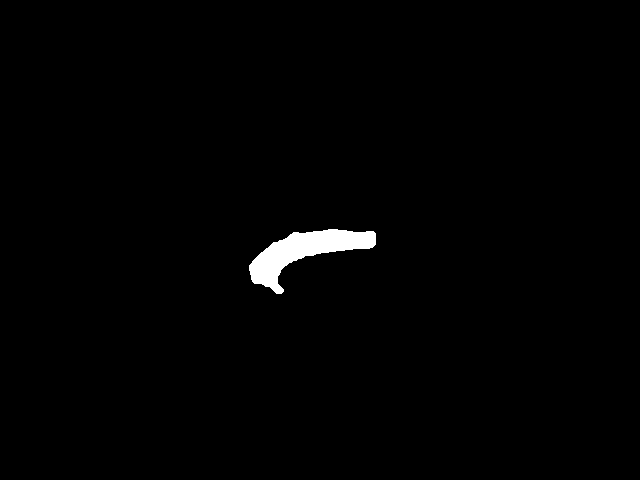
\includegraphics[width=\textwidth]{banana_1_1_100_mask}
		\caption{Banana - mask}
	\end{subfigure}
	
	\caption{Two samples of Washington dataset}
	\label{fig:washington_samples}
\end{figure}

For our software platform, we intend on using Keras, a Python wrapper for neural
networks. Keras was originally designed to use Theano as a backend, but it is
easily extensible and can be used with TensorFlow as a backend without too much
additional work. No outside code other than pretrained ImageNet network model
weights will be used.


\section{Reservations}

As far as anticipated stumbling blocks are concerned, our only immediate worry
is training time. In order to achieve results similar to our reference paper,
even using pretrained networks, we will have to spend significant CPU time. We
have a new machine we can use for training, but one machine is not equivalent to
a server farm or paid AWS instances.

Otherwise, we feel confident with our approach. Our dataset is straight-forward
to use and pre-segmented. Keras is also an easy-to-use software package.


\section{Relationship to your Background}

As mentioned earlier, we are both first-year graduate students under Professor
Minh Do. Between the two of us, we have extensive software engineering experience, but neither of us have done any work with deep learning or object recognition in the past. In particular, Dario has used Keras for a toy project in the past, but only used it for a simple fully-connected neural network.

This project will be the first step in Mac's PhD thesis, but it has no relation to Dario's research. 


\bibliographystyle{abbrv}
\bibliography{mybib}


%%% End document
\end{document}